\documentclass[english,11pt,aspectratio=1610,xcolor=table]{beamer}
\input{setup/setup}
\input{setup/setup-colors}
\input{setup/setup-settings}

\usetheme{JD}
\beamertemplatenavigationsymbolsempty
% header fields: usage
% \field
%     [short form (footline)]
%     {long form on title page}
%
\title
    [Testing of software that implements logical systems]
    {Testing of software that implements logical systems}

\subtitle{Final presentation} % short version unused by this template
\author
    [Tamás Karcag]
    {Tamás Karcag}
\institute
    [\hypersetup{urlcolor=jdgrey}%
     \href{https://www.elte.hu/}{ELTE} %
     \href{https://www.inf.elte.hu/}{IK} %
     \href{http://compalg.inf.elte.hu/}{COMP}]
    {Komputeralgebra\\%
     Faculty of Informatics\\%
     Eötvös Loránd University}
\date
    [01/2025]
    {13 January 2025}

\begin{document}

\maketitle

\begin{frame}{Outline}
    \tableofcontents
\end{frame}

\subsection{Background and Motivation}
\begin{frame}{Introduction}
    \begin{alertblock}{Background and Motivation}
        \begin{itemize}[<+->]\itemsep9pt
            \item \textbf{Evolving Digital Landscape}: Increased focus on security and reliability.
            \item \textbf{Software Testing}
                \begin{itemize}
                    \item Ensuring the \textbf{correctness} of \textbf{complex business logic}.
                    \item Increase \textbf{accuracy} and \textbf{reliability}.
                    \item \textbf{Incomplete tests} can lead to \textbf{undetected defects}.
                \end{itemize}
            \item \textbf{Cause-Effect Graphs in Testing}
                \begin{itemize}
                    \item \textbf{Model business logic}.
                    \item Visualize \textbf{causes} and their \textbf{effects}.
                    \item Test case generation: \textbf{manual}, \textbf{inefficient}, and lack \textbf{scalability}.
                \end{itemize}
        \end{itemize}
    \end{alertblock}
\end{frame}
\begin{frame}{Problem Statement}
    \begin{alertblock}{Challenges in Testing Complex Systems}
        \begin{itemize}[<+->]\itemsep9pt
            \item Ensuring \textbf{business logic accuracy} is difficult.
            \item Providing testing \textbf{completeness} and \textbf{scalability}.
        \end{itemize}
    \end{alertblock}

    \begin{alertblock}{Cause-Effect Graphs}
        \begin{itemize}[<+->]\itemsep9pt
            \item \textbf{Strengths}: 
                \begin{itemize}
                    \item \textbf{Structured} and \textbf{visualized} representation.
                    \item Aid in \textbf{understanding} and modeling complex dependencies.
                \end{itemize}
            \item \textbf{Challenges}:
                \begin{itemize}
                    \item Transitioning from \textbf{visual} cause-effect graphs to \textbf{actionable} test cases.
                    \item Automatization, scaling and reusing.
                \end{itemize}
        \end{itemize}
    \end{alertblock}
\end{frame}
\begin{frame}{Literature Review}

\end{frame}
\begin{frame}{Metholodgy}

\end{frame}
\subsection{Application Architecture}
\begin{frame}{Application Architecture}
    \center
    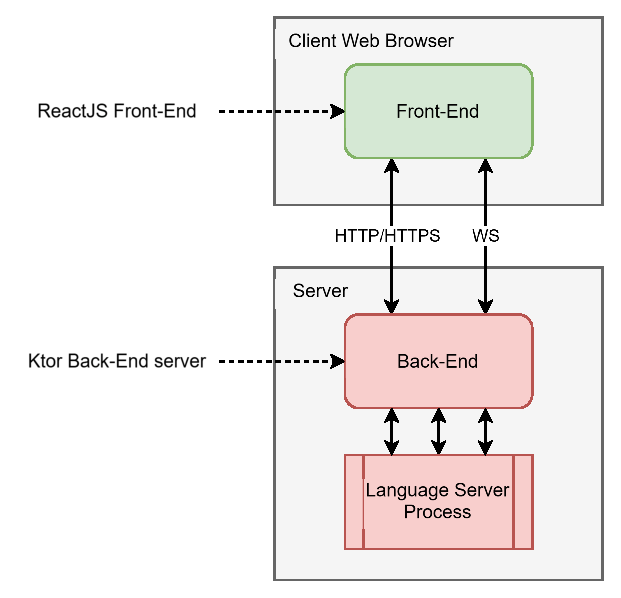
\includegraphics[height=240px]{images/AppArch}
\end{frame}

\begin{frame}{Application Architecture}
    \begin{alertblock}{Architecture}
        \begin{itemize}[<+->]\itemsep9pt
            \item Modular React Front-End
                \begin{itemize}
                    \item Intuitive \textbf{graph visualization}.
                    \item Real-time \textbf{syntax highlighting} and \textbf{error feedback}.
                \end{itemize}
            \item Back-End
                \begin{itemize}
                    \item Implements \textbf{core business logic}: complex rule handling and transformation.
                    \item Seamless conversion into decision tables and optimized outputs.
                    \item Manages communication with \textbf{Kotlin Language Server}.
                    \item Custom graph language developed using \textbf{Kotlin's DSL} capabilities
                \end{itemize}
        \end{itemize}
    \end{alertblock}
    \begin{alertblock}{Deployment Infrastructure}
        \begin{itemize}[<+->]\itemsep9pt
            \item Automatization via \textbf{Dockerized} environment and \textbf{Azure} DevOps pipelines.
        \end{itemize}
    \end{alertblock}
\end{frame}
\begin{frame}{Architecture Overview}
    \begin{alertblock}{Backend}
        \begin{itemize}[<+->]\itemsep9pt
            \item Built with Kotlin and Ktor framework.
            \item Handles REST API, WebSocket communication, and logical transformations.
        \end{itemize}
    \end{alertblock}
    \begin{alertblock}{Frontend}
        \begin{itemize}[<+->]\itemsep9pt
            \item Developed in ReactJS for intuitive graph creation and visualization.
        \end{itemize}
    \end{alertblock}
    \begin{alertblock}{Integration}
        \begin{itemize}[<+->]\itemsep9pt
            \item Kotlin Language Server for parsing and validation.
        \end{itemize}
    \end{alertblock}
\end{frame}
\begin{frame}{Results}
    \begin{alertblock}{Performance Efficiency}
        \begin{itemize}[<+->]\itemsep9pt
            \item Efficient performance even with large datasets, though slow client-side rendering for large results.
        \end{itemize}
    \end{alertblock}
    \begin{alertblock}{Transformation Accuracy}
        \begin{itemize}[<+->]\itemsep9pt
            \item 100\% accuracy for simple rules with a single cause.
            \item Reliable transformations for nested rules and logical operators (AND, OR, NOT).
            \item Effective error handling with clear notifications for syntax and logical errors.
        \end{itemize}
    \end{alertblock}
\end{frame}

\begin{frame}{Results}
    \begin{alertblock}{Scalability and Responsiveness}
        \begin{itemize}[<+->]\itemsep9pt
            \item Concurrent Usage: Handles moderate user concurrency with minimal delay.
            \item Performance drops with high concurrency (50+ simultaneous sessions), indicating need for further scalability solutions.
        \end{itemize}
    \end{alertblock}
    \begin{alertblock}{Usability}
        \begin{itemize}[<+->]\itemsep9pt
            \item Intuitive user interface with real-time error notifications.
            \item Easy transformation from cause-effect graphs to decision tables and test cases.
        \end{itemize}
    \end{alertblock}
\end{frame}
\begin{frame}{Challenges}

\end{frame}
\begin{frame}{Contributions}

\end{frame}
\chapter{Conclusion}
\label{ch:conclusion}

In conclusion, this thesis will summarize the contributions, highlight key limitations, and outline potential future directions for the project.

\section{Summary of Contributions}

This project aimed to develop a comprehensive application that supports users in defining, visualizing, and transforming cause-effect relationships through an intuitive front-end interface and a robust back-end logic processing system. Major contributions include the creation of a custom graph-based language, built on Kotlin's DSL capabilities, which allows for the flexible modeling of logical rules. Additionally, a modular React front-end was developed to provide an interactive and user-friendly experience, supported by server-side processing. The development process is automated using Azure Pipelines, and the application is deployed via Docker, ensuring scalability and streamlined deployment.

This architecture and toolset effectively support the seamless conversion of rule definitions into logical formulas, decision tables, and optimized outputs for test generation, providing a strong foundation for further development and testing.

\section{Limitations}

While the application effectively meets the primary objectives, several limitations exist. 

\begin{itemize}
    \item First and foremost, it currently lacks persistent data storage, limiting the ability to save user progress and historical data for future work sessions and reuse. 
    \item Moreover, although the language server integration is operational, it could be improved with further refinements to enhance syntax support, error handling, and helpful hints in the editor.
    \item Lastly, addressing scaling challenges for high concurrent usage and more extensive client-server interactions presents opportunities for future enhancements. Upgrading the deployment platform and automation processes will be essential for achieving a more scalable infrastructure. Kubernetes and load balancers could serve as effective solutions to address this limitation.
\end{itemize}

\section{Future Work}

Future development aims to extend the application's capabilities and address current limitations. 

Planned enhancements include implementing persistent data storage to allow users to save and retrieve graph definitions and transformation histories. Currently, the application lacks user registration and management capabilities. To offer a more personalized experience, future updates should include features for user account creation, authentication, and management. Additionally, implementing work session management will allow users to save and resume their progress across sessions, making the application more user-friendly and adaptable to collaborative or extended projects. This enhancement would pave the way for more robust user-specific data handling, facilitating a tailored and secure user experience.

Improving processing capacity is crucial for handling more complex models and managing larger datasets efficiently in a concurrent manner. While this largely depends on hardware capabilities, the software already features a lightweight, optimized codebase with essential functionality in place. Automatic scaling could be effectively implemented using Kubernetes or similar advanced cloud solutions.

The application's editor currently offers IntelliSense features for code editing, including real-time syntax checking. To create a more robust solution, the editor should also alert users to semantic issues during code editing or prior to execution, rather than only after execution.

Closer integration with automated test generation tools would significantly enhance efficiency. Establishing a streamlined process for exporting results to external tools will further improve the application's utility in development and testing environments.
\subsection{Questions}
\begin{frame}{Questions?}
Thank the audience and open the floor for questions.
\end{frame}
\end{document}